\chapter{Studi Literatur}

\par Pada bab ini dipaparkan hasil studi literatur terkait dengan sistem competitive programming. Studi literatur yang dilakukan adalah terkait sistem yang digunakan dalam menyelenggarakan kompetisi competitive programming, online judging system, auto grader dan metode yang digunakan dalam melakukan grading.

\section{Competitive Programming}

\par Competitive programming merupakan sebuah kompetisi dimana peserta dari kompetisi tersebut diminta menyelesaikan suatu permasalahan pada bidang computer science secara cepat dan tepat. Pada kompetisi competitive programming, peserta akan diberikan permasalahan computer science yang sudah pernah diselesaikan dan bukan permasalahan riset yang solusinya masih belum ditemukan (\cite{halimsfcp3}). Untuk setiap persoalan yang diberikan, peserta diminta untuk menyelesaikan masalah tersebut dengan membuat program dalam bahasa pemrograman yang diizinkan oleh juri. Program yang dibuat oleh peserta harus memenuhi batasan yang dibuat oleh juri seperti waktu eksekusi, kebutuhan memori, dan ukuran program.
\par Pada kompetisi competitive programming, program yang telah dibuat oleh peserta akan dinilai dengan suatu metode tertentu. Umumnya penilaian yang dilakukan mencakup kebenaran program dan waktu pengumpulan program, akan tetapi terdapat beberapa metode penilaian lain yang dapat dilakukan. Beberapa standar metode telah digunakan untuk melakukan penilaian jawaban dalam kompetisi competitive programming, diantaranya adalah standar IOI dan ICPC. Beberapa kompetisi competitive programming diselenggarakan oleh suatu organisasi, contohnya adalah ICPC yang diselenggarakan oleh ICPC Foundation (About ICPC, 2018), dan IOI (International Olympiad in Informatics) yang diselenggarakan oleh IOI Community (Organization, Desember 19 2017). Selain itu, terdapat juga kompetisi competitive programming yang diselenggarakan oleh suatu perusahaan seperti Google Code Jam yang diselenggarakan oleh Google dan Facebook HackerCup yang diselenggarakan oleh Facebook.
\par Kompetisi competitive programming pada tingkat perguruan tinggi biasanya mengikuti standar ICPC. Beberapa kompetisi yang mengikuti standar ini adalah Gemastik, Compfest, Vocomfest, INC, dan ACM-ICPC. Pada standar ICPC, setiap peserta akan bekerja dalam sebuah tim yang terdiri dari tiga peserta. Tiap tim akan diberikan soal yang sama. Seluruh tim akan mulai mengerjakan soal secara bersama-sama. Program yang telah dibuat oleh sebuah tim akan dikirimkan ke sistem untuk dinilai. Penilaian dilakukan secara otomatis pada sistem yang disebut online judge. Pada sistem online judge penilaian dilakukan dengan menggunakan sebuah autograder yang berjalan di dalam sistem online judge, autograder akan menjalankan program yang dikirimkan oleh peserta dan menentukan apakah program tersebut benar atau salah. Setiap program yang dikirimkan oleh peserta hanya dapat bernilai benar atau salah. Setiap tim yang mengirimkan program yang salah akan mendapatkan penalti waktu. Nilai total dari sebuah tim dihitung dari jumlah soal yang berhasil dikerjakan oleh tim tersebut. Jika terdapat dua buah tim yang menyelesaikan soal dengan jumlah yang sama akan dihitung jumlah penalti waktunya untuk menentukan tim yang nilainya lebih tinggi (World Finals Rules for 2019, 4 Oktober 2018).
\par Selain standar ICPC, terdapat standar lain yang biasa digunakan untuk tingkat sekolah menengah atas yaitu standar IOI. Pada standar IOI setiap peserta bekerja secara individu dan mendapatkan soal yang sama. Berbeda dengan standar ICPC, pada standar IOI setiap soal memiliki beberapa subtask dengan nilai tertentu. Peserta dapat menyelesaikan soal secara parsial dan mendapatkan nilai berdasarkan total dari subtask yang berhasil diselesaikan dengan benar pada soal tersebut (IOI 2017 Contest Rules, 2018).
\par Terdapat jenis competitive programming lain yang tidak memiliki standar tertentu, misalnya Google Code Jam dan Codeforces. Pada kompetisi Google Code Jam, sistem tidak melakukan penilaian dengan menjalankan program yang dibuat oleh peserta, melainkan hanya meminta jawaban dari peserta dalam bentuk file output yang sudah dihasilkan oleh program peserta yang dijalankan di komputer peserta sendiri. Pada kompetisi Codeforces, sistem penilaian memiliki banyak perbedaan dengan sistem penilaian lain. Pada kompetisi ini, setiap soal memiliki nilai yang berbeda dan nilainya akan terus berkurang selama kompetisi berlangsung. Selain itu, pada kompetisi Codeforces peserta dapat melakukan hack pada program yang telah dikirimkan peserta lain (Codeforces Contest Rules, 2011).

\section{Online Judge System}

\par Online judge merupakan suatu platform yang digunakan untuk menyelenggarakan kompetisi competitive programming. Peserta kompetisi menggunakan online judge system untuk mengakses soal dan mengirimkan jawaban atau program yang telah dibuat. Online judge system akan melakukan kompilasi pada kode yang dikirimkan peserta lalu mengevaluasi program yang dihasilkan dengan test case tertentu untuk menilai jawaban peserta tersebut (Wasik, Antczak, Badura, Laskowski, \& Sternal, 2018). Selain itu online judge system juga memiliki beberapa fungsi lain diantaranya adalah untuk melihat scoreboard dan melakukan klarifikasi pada soal. Umumnya online judge system berupa halaman web yang berisi antar muka untuk membaca soal dan mengirimkan jawaban dari soal tersebut. Gambar \ref{fig:codeforces} memperlihatkan contoh halaman soal dari sistem online judge yang cukup populer yaitu Codeforces.

\begin{figure}
	\centering
	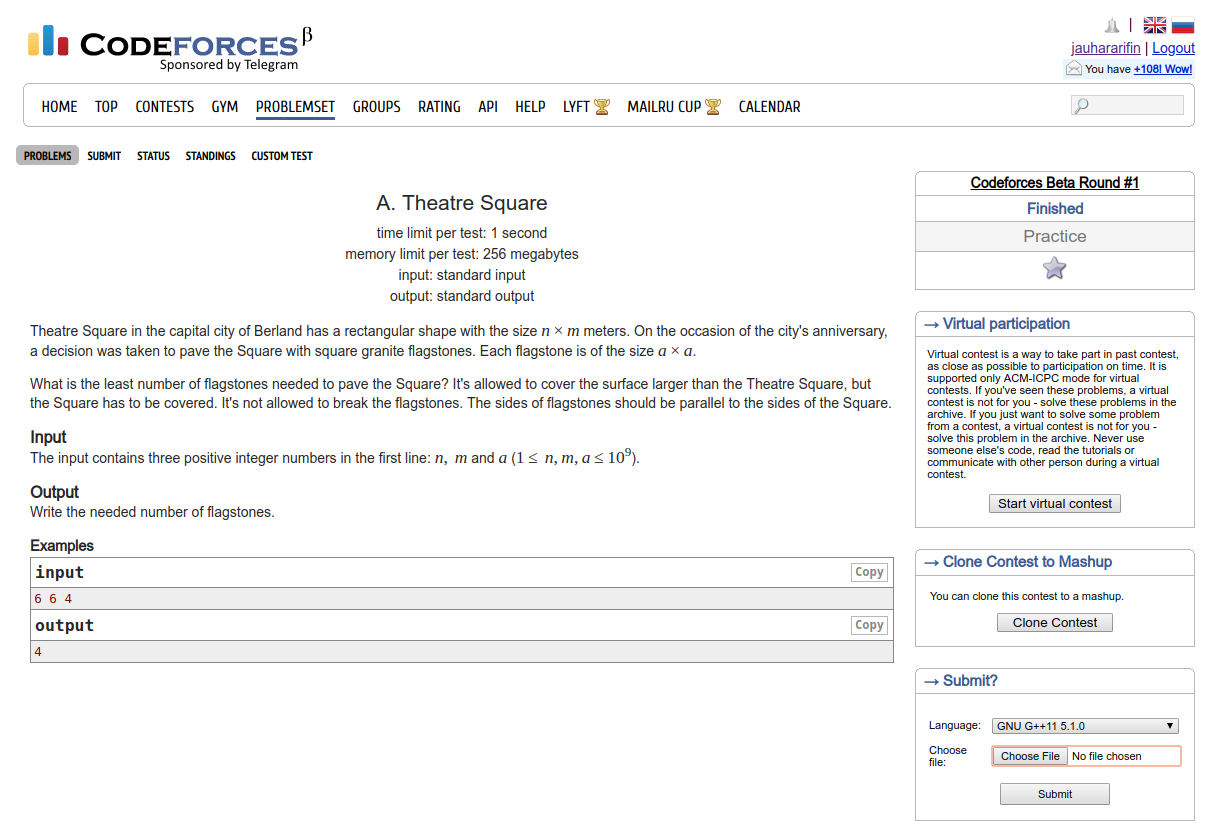
\includegraphics[width=\textwidth]{images/codeforces}
	\caption{Contoh Online Judge System : Codeforces.}
	\label{fig:codeforces}
\end{figure}

\par Beberapa organisasi memiliki online judge yang secara publik dapat diakses, diantaranya adalah: URI Online Judge, TOKI Online Judge, Codeforces, Uva, SPOJ, dan lain sebagainya. Online judge yang bersifat publik ini biasanya memiliki beberapa soal-soal yang dapat digunakan untuk latihan dan dapat dikerjakan tanpa harus berkompetisi dengan peserta lain. Pada URI Online Judge terdapat fitur tambahan seperti forum dan rewarding system (\cite{uriojpaper}). Terdapat beberapa sistem online judge yang bersifat open source seperti Mooshak, Judgels, dan DomJudge. Sistem online judge yang bersifat open source biasanya digunakan untuk oleh beberapa instansi seperti universitas untuk membuat kompetisi competitive programming yang bersifat privat seperti Gemastik, Compfest, Vocompfest, Arkavidia, dan INC.

\section{Autograder}

\par Autograder merupakan suatu aplikasi yang digunakan untuk melakukan kompilasi, eksekusi dan menilai sebuah source code (Danutama \& Liem, 2013). Autograder digunakan dalam sistem online judge untuk menilai kebenaran suatu source code. Umumnya autograder akan melakukan kompilasi pada source code yang dikirimkan oleh peserta pada kompetisi competitive programming. Hasil kompilasi dari kode peserta tersebut akan di-test dengan menggunakan test-case rahasia yang telah dibuat oleh juri atau problem setter. Setelah melalui pengetesan, program akan dinilai berdasarkan hasil pengetesan tersebut. Gambar \ref{fig:grading-process} menjelaskan alur penilaian sebuah source code yang dikirimkan peserta.

\begin{figure}
	\centering
	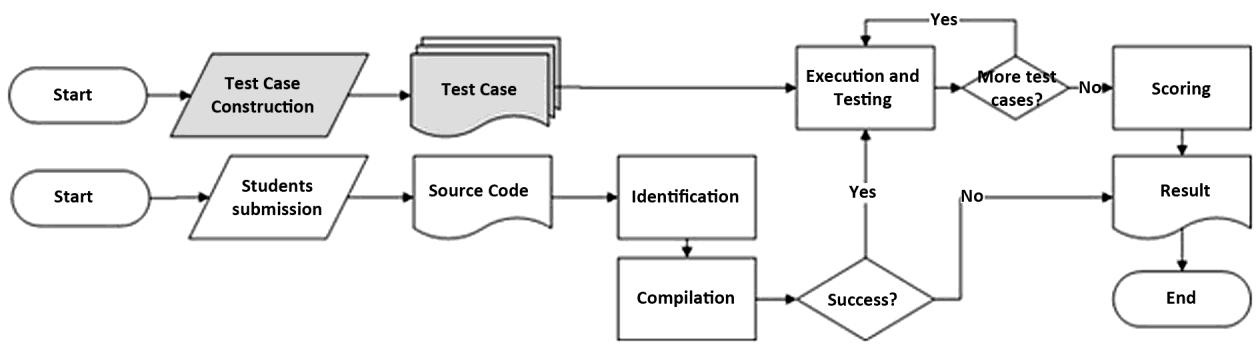
\includegraphics[width=\textwidth]{images/grading-process}
	\caption{Proses penilaian program peserta (Danutama \& Liem, 2013).}
	\label{fig:grading-process}
\end{figure}

\par Seluruh proses penilaian sebuah source code peserta membutuhkan waktu tiga menit jika dilakukan secara manual, sedangkan hanya membutuhkan waktu sepuluh detik dengan menggunakan autograder (Danutama \& Liem, 2013). Dengan menggunakan autograder, peserta kompetisi competitive programming dapat menerima feedback dengan lebih cepat dan mengurangi pekerjaan yang harus dilakukan oleh juri.

\par Terdapat banyak hal yang harus diperhatikan dalam membangun sistem online judge dengan menggunakan autograder. Salah satu permasalahan yang harus dihadapi dalam membangun autograder adalah masalah keamanan sistem. Sistem autograder harus dapat bertahan terhadap serangan yang mungkin dilakukan oleh peserta. Beberapa serangan yang mungkin dilakukan oleh peserta adalah mengirimkan source code yang memiliki waktu kompilasi yang sangat lama dan membebani sistem, membuat kode yang dapat mengubah atau merusah lingkungan testing autograder, dan mengakses resource dari autograder yang tidak diizinkan oleh sistem (Wasik, Antczak, Badura, Laskowski, \& Sternal, 2018). Metode yang mungkin dilakukan untuk mengatasi masalah keamanan tersebut adalah dengan melakukan sandboxing. Sandboxing merupakan teknik mengisolasi suatu eksekusi program sehingga tidak mengganggu lingkungannya. Metode sandboxing yang populer untuk masalah ini adalah dengan menggunakan virtualization seperti KVM, atau menggunakan container seperti LXC dan Docker.

\par Hal lain yang perlu diperhatikan dalam membangun autograder adalah fairness. Waktu eksekusi program perlu diukur dengan tepat untuk menciptakan sistem yang adil. Waktu eksekusi program yang sama dengan input yang sama dapat memiliki nilai yang berbeda bergantung beberapa faktor seperti kecepatan CPU, ukuran RAM, dan lain sebagainya. Waktu pengukuran sebuah program dalam sistem autograder biasanya dilakukan dalam hitungan milidetik. Beberapa metode yang dapat digunakan untuk mengukur waktu pemrosesan adalah dengan melakukan analisis pada hardware performance, code instrumentation, atau code sampling (Wasik, dkk., 2018). Umumnya autograder dalam sebuah sistem online judge memiliki banyak worker untuk meningkatnya banyaknya program yang dapat dinilai dalam satuan waktu. Autograder ini dapat dijalankan di komputer yang berbeda, dan dapat memiliki kinerja yang berbeda. Oleh karena itu, pengukuran waktu sangat penting dalam sistem autograder untuk meningkatkan fairness dari sistem.

\section{Containerization}

\par Secara singkat container merupakan teknologi virtualisasi program pada level sistem operasi, berbeda dengan teknik virutalisasi menggunakan hypervisor yang bekerja pada level hardware (Merkel, 2014). Container bekerja seperti virtual machine yang dapat memberikan isolasi terhadap program yang berjalan. Pada virtual machine, virtualisasi terjadi pada level hardware sehingga pengguna perlu menginstall sistem operasi pada lingkungan yang terisolasi untuk dapat menjalankan program. Pada container, pengguna tidak perlu menginstall sistem operasi karena virtualisasi terjadi pada level software sehingga sistem operasi dari host dapat digunakan dalam container. Hal tersebut membuat container lebih ringan dibandingkan virtual machine karena tidak ada overhead untuk menjalankan sistem operasi baru. Gambar \ref{fig:docker-architecture} mengilustrasikan arsitektur salah satu container yang populer yaitu Docker.

\begin{figure}
	\centering
	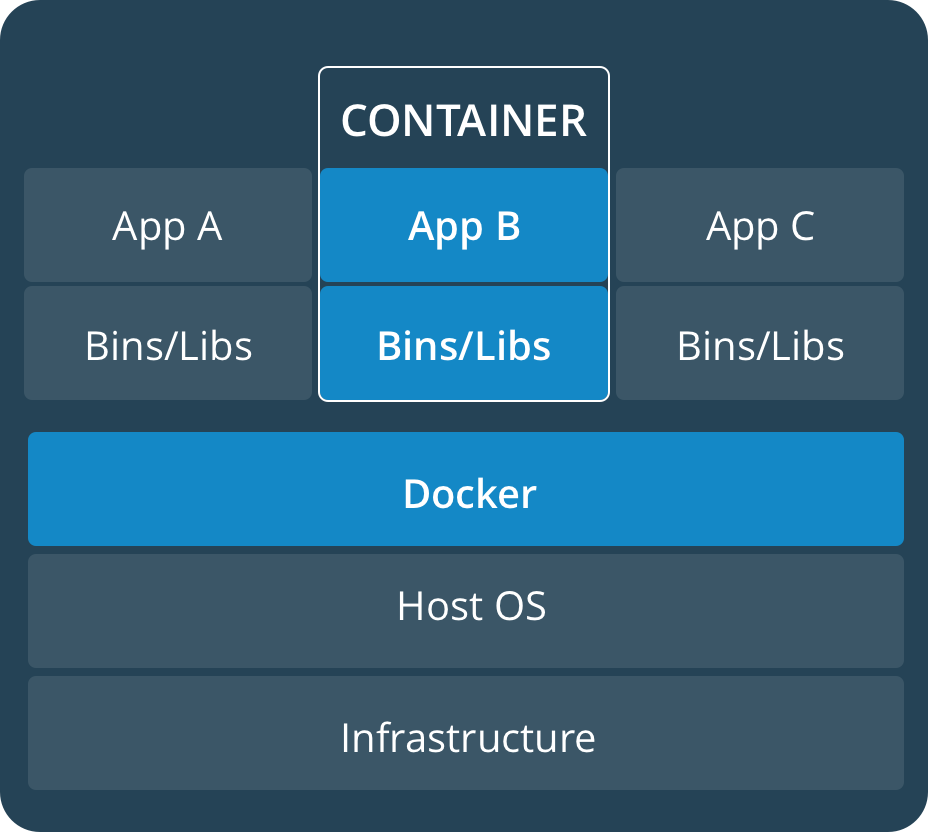
\includegraphics[width=0.5\textwidth]{images/docker-architecture}
	\caption{Arsitektur container pada Docker (Docker Documentation, 2018).}
	\label{fig:docker-architecture}
\end{figure}

\par Pada linux, teknologi mungkin dilakukan karena adanya beberapa fitur dari linux yaitu: chroot, cgroup dan namespace. Cgroup dapat memberikan isolasi file system terhadap suatu program yang berjalan pada linux. Cgroup dapat memberikan batasan resource kepada suatu program yang berjalan pada linux. Namespace dapat memberikan isolasi pada program sehingga program dalam suatu lingkungan tidak dapat mengetahui adanya program pada lingkungan lain. Terdapat beberapa perangkat lunak yang menawarkan teknologi containerization ini, yang populer diantaranya adalah: Docker dan LXC. Dengan menggunakan Docker atau LXC, pengguna dapat membuat suatu lingkungan yang tersiolasi untuk menjalankan suatu program tertentu tanpa mengganggu lingkungan diluar lingkungannya. Docker memberikan API yang lebih high-level dibandingkan dengan LXC, dan memiliki banyak fitur yang dapat digunakan untuk mengelola container. Docker biasanya digunakan sebagai platform untuk mendeploy aplikasi.

\par Teknologi container dapat digunakan untuk melakukan penilaian terhadap kode program yang dikirimkan oleh peserta kompetisi competitive programming. Dengan menggunakan container, program yang dijalankan dapat diisolasi sehingga tidak membahayakan lingkungan. Selain itu, resource seperti CPU usage, memory, storage, dan IO pada container dapat dibatasi sehingga tidak mengganggu program lain yang sedang berjalan pada lingkungan di luar container (Merkel, 2014).

\section{Chroot}

\par Chroot merupakan system call pada sistem operasi yang berbasis linux atau unix. System call ini dapat mengubah root filesystem ke direktori target tertentu kemudian menjalankan program. Program yang dijalankan seakan-akan memiliki direktori root sebagai direktori yang dispesifikasi pada waktu pemanggilan system call chroot. Dengan mengguakan cara ini, program yang dijalankan dalam chroot hanya dapat mengakses filesystem yang berada pada direktori target saja dan mengurangi kemungkinan serangan yang mungkin dilakukan pada filesystem asli (Lessard, 2003). Dengan menggunakan chroot, pengguna dapat mengatur library apa saja yang dapat digunakan oleh program yang berjalan dalam lingkungan chroot. Hal ini dapat menjadi merepotkan karena pengguna perlu memasukkan semua library yang dibutuhkan ke dalam filesystem chroot. Teknologi container memanfaatkan chroot untuk mengisolasi filesystem yang dapat diakses oleh program yang berjalan pada container.

\par Meskipun chroot memberikan penghalang pada aplikasi yang berada dalam lingkungan chroot untuk mengakses filesystem yang berada di luar lingkungan direktori target, chroot masih memiliki kelemahan. Jika aplikasi yang berjalan pada lingkungan chroot memiliki root permission, maka aplikasi tersebut dapat dengan mudah keluar dari lingkungan chroot. Terdapat beberapa cara untuk meningkatkan keamanan chroot sehingga program yang berjalan di dalam chroot sulit  untuk keluar dari lingkungan tersebut.

\par Salah satu cara untuk meningkatkan keamanan pada lingkungan chroot adalah dengan memasukkan file yang hanya dibutuhkan oleh program saja. Sebagai contoh, jika program membutuhkan daftar user yang berada dalam sistem, di dalam linkungan chroot perlu ada file /etc/passwd untuk mendapatkan informasi ini. Akan tetapi, file /etc/shadow tidak perlu dimasukkan ke dalam filesystem chroot karena mengandung informasi rahasia yang tidak diperlukan oleh program yang berada dalam lingkungan chroot.

\par Cara kedua untuk meningkatkan keamanan lingkungan chroot adalah dengan tidak memberikan akses root kepada program yang berjalan di dalam chroot. Terdapat beberapa serangan yang memungkinkan program dalam lingkungan chroot untuk keluar dari lingkungan chroot jika memiliki akses root. Untuk menghindari jenis serangan ini, sebaiknya program yang berjalan di dalam lingkungan chroot dibuat agar tidak mungkin mendapatkan akses root. Tidak memberikan akses root kepada program akan mengurangi kemungkinan adanya serangan. Akan tetapi, meskipun tidak memberikan akses root, masih terdapat beberapa serangan yang memungkinkan program membangkitkan akses root tanpa memiliki akses root pada saat dijalankan.

\par Untuk meningkatkan keamanan pada lingkungan chroot, sebaiknya tidak memasukkan hard link ke dalam filesystem chroot. Hard link yang mengacu pada file di luar lingkungan chroot akan mengurangi keamanan chroot karena memungkinkan program yang berada di dalam lingkungan chroot untuk mengakses file yang berada di luar lingkungan chroot.

\section{Cgroup}

\par Cgroup merupakan fitur pada linux yang dapat digunakan untuk membatasi resource yang digunakan oleh suatu kelompok program (Felter, Ferreira, Rajamony, \& Rubio, 2014). Resource yang dimaksud di sini adalah CPU usage, memory usage, disk IO dan network IO. Dengan menggunakan cgroup, sebuah program yang dibatasi resource-nya tidak akan mengganggu program lain dengan cara menghabiskan resource. Fitur cgroup dimanfaatkan oleh teknologi container untuk membatasi resource pada sebuah container sehingga tidak membebani program lain di luar container. Pada container, umumnya cgroup digunakan untuk membatasi CPU dan memory yang digunakan oleh program-program yang berjalan di dalam container. Cgroup dapat memberhentikan program di dalam container jika telah menggunakan resource yang berlebihan.

\section{Namespace}

\par Dengan menggunakan chroot dan cgroup, sebuah program dapat diisolasi sehingga memiliki resource dan filesystem sendiri yang terpisah dari program-program lain yang berjalan pada host operating system. Meskipun begitu, program yang terisolasi ini masih dapat melihat proses apa saja yang sedang berjalan pada sistem operasi karena program yang berjalan di dalam chroot dan cgroup masih menggunakan sistem operasi yang sama dan menggunakan kernel yang sama. Linux memiliki fitur namespace yang memberikan isolasi kepada program terhadap masalah ini. Dengan menggunakan namespace, sebuah program dapat berjalan di atas namespace tertentu dan hanya dapat mengetahui program lain yang berada di dalam namespace yang sama. Pada container, namespace digunakan sehingga program yang berjalan di dalam container hanya mengetahui program yang berada di dalam container tersebut dan tidak dapat mengetahui program yang sedang berjalan pada host OS-nya (Felter dkk., 2014).

\par Selain isolasi program, namespace juga memberikan isolasi pada hal lain seperti network, mount, cgroup, user, dan lain sebagainya. Dengan memberikan isolasi pada network, program yang berada di dalam container dapat membuka port yang sama seperti program lain yang berada di container lain. Dengan menggaunakan isolasi pada user, user yang ada di dalam container tidak dapat diketahui oleh container lain.

\section{Kernel Virtual Machine}

\par Virtual machine memberikan teknik virtualisasi yang berbeda dengan container. Container berjalan pada level sistem operasi sedangkan virtual machine berjalan pada level hardware. Pada container, fitur-fitur dari linux digunakan untuk mendukung virtualisasi dan isolasi program, sedangkan pada virtual machine digunakan hypervisor untuk melakukan virtualisasi. Dengan menggunakan virtual machine, pengguna dapat menjalankan lebih dari satu sistem operasi berbeda di dalam komputer yang sama berbeda dengan container yang hanya dapat menjalankan satu sistem operasi saja. KVM merupakan fitur dari linux yang memungkinkan linux menjadi hypervisor dan menjalankan guest OS di dalam proses linux (Felter et al., 2014).

\par KVM memiliki fitur yang mirip dengan container. Program yang berjalan di dalam virtual machine terisolasi dari program yang ada di luar-nya. Resource pada program yang berjalan di virtual machine juga dapat dibatasi. Berbeda dengan container, program yang berjalan di atas virtual machine dikelola oleh sistem operasi yang berjalan di virtual machine tersebut. Dengan menggunakan KVM, pengguna dapat menjalankan sistem yang benar-benar berbeda dengan linux, tidak seperti container yang hanya dapat menjalankan program yang berarsitektur linux. Virtual machine lebih berat dibandingkan container karena untuk menjalankan program pada virtual machine diperlukan sistem operasi sendiri yang berjalan yang mengakibatkan adanya overhead untuk booting, manajemen memori, manajemen proses, scheduling, dan lain sebagainya.

\par KVM tidak cocok untuk digunakan dalam autograder karena terlalu banyak overhead yang diperlukan dan memberatkan sistem. Untuk mengevaluasi source code peserta, tidak perlu menggunakan sistem operasi sendiri yang berbeda dengan sistem operasi yang menjalankan sistem autograder. Dalam pembuatan autograder, penggunaan teknologi container lebih cocok untuk digunakan dibandingkan dengan penggunaan teknologi virtual machine. Virtual machine lebih cocok digunakan untuk melakukan pengetesan program yang membutuhkan berbagai macam sistem operasi. Selain itu virtual machine juga kerap digunakan dalam pembuatan sistem IaaS seperti Amazon EC2, Digital Ocean Droplet dan Google Cloud Compute Engine.

\section{WebAssembly}

\par WebAssembly merupakan WebAPI yang memungkinkan browser untuk menjalankan low-level code secara aman. Dulunya Javascript merupakan satu-satunya bahasa yang dissuport secara native oleh web, akan tetapi semakin berkembangnya teknologi web kebutuhan akan performa dari web semakin tinggi. Javascript yang merupakan interpreted language tidak dapat memberikan performa yang tinggi seperti bahasa-bahasa yang dikompilasi menjadi low-level code. WebAssembly memberikan solusi yang memungkinkan browser untuk menjalankan low-level code pada sebuah sistem yang terisolasi dan aman. WebAssembly didesain untuk digunakan bersama-sama dengan Javascript untuk mengembangkan aplikasi web. Sebuah aplikasi web dapat memanfaatkan WebAssembly untuk meningkatkan kinerja dan memanfaatkan Javascript untuk fleksibilitas (WebAssembly, 2018).

\par Dengan menggunakan WebAssembly, browser dapat membuat sebuah lingkungan yang terisolasi untuk menjalankan low-level code. Lingkungan yang digunakan untuk menjalankan kode WebAssembly memiliki beberapa batasan seperti jumlah memori yang bisa digunakan, file yang bisa diakses dan lain sebagainya. Umumnya kode WebAssembly hanya dapat melakukan apa yang dapat dilakukan oleh web. Web tidak dapat mengakses sembarang file yang berada pada komputer, begitu juga WebAssembly. Web tidak dapat melakukan beberapa system call, begitu juga WebAssembly. Meskipun WebAssembly dapat melakukan isolasi pada program yang berjalan, pembatasan resource pada WebAssembly masih sulit dan tidak semudah dengan menggunakan container ataupun virtual machine. 

\par Kode WebAssembly berupa binary code yang dapat dibuat dengan cara melakukan kompilasi dari beberapa bahasa seperti C, C++ dan Rust ke dalam format wasm. WebAssembly masih baru dan belum banyak bahasa pemrograman yang dapat dikompilasi menjadi WebAssembly. Bahasa pemrograman yang menggunakan interpreter atau runtime environment seperti Python dan Java masih sulit dijalankan di dalam WebAssembly.

\par Dalam sistem autograder, WebAssembly tidak cocok digunakan karena berbagai alasan, yaitu: masih sedikitnya bahasa pemrograman yang dapat dikompilasi menjadi kode WebAssembly, sulitnya membatasi resource pada WebAssembly, sulitnya melakukan perhitungan waktu, dan sulitnya menjaga keamanan. Browser yang ada pada saati ini memiliki kemampuan untuk mengubah kode Javascript yang berjalan pada browser tersebut, hal ini mengakibatkan munculnya celah keamanan pada WebAssembly jika digunakan untuk mengevaluasi kode peserta.
